\chapter{Defining refactoring-oriented clone types}\label{chap:clonetypes}
In section \ref{chap:backgroundclonetypes} we introduced the four clone types as defined in literature. These simple definitions are suitable for analysis of a codebase. Their detection results in simple to understand numbers to argue about a codebase. However, these clone types have a few flaws which makes it hard to argue to what extend two fragements of code are functionally related. For each of type 1-3 clones~\cite{roy2007survey} we list our solutions to their shortcomings to increase the chance that we can refactor the clone while improving the design. Due to the serious challenges involved in their detection and refactoring, type 4 clones are not considered in this study.

We also look into clone detection tools for their suitability to support the proposed clone type definitions. We selected a few criteria  Most clone detection tools support these definitions of clone types. However, many of these tools use a vastly different approach. A study by Saini et al \cite{saini2018towards} outlines different clone detection tools and compares their results for each of type 1-3 clones. Even though they operate on the same type definitions, the tools used in this study yield different results.

\section{Shortcomings of clone types}
The clone definitions, as outlined in section \ref{chap:backgroundclonetypes}, allow reasoning about the duplication in a software system. Clones by these definitions can relatively easily and efficiently be detected. This has allowed for large scale analyses of duplication. However, these clone type definitions have shortcomings which makes the clones detected in correspondance with these definitions less valuable for (automated) refactoring purposes.

In this section we discuss the shortcomings of the different clone type definitions which make them less suitable for (automated) refactoring. Because of that, these clones require more judgement whether they should and can be refactored.

\subsection{Type 1 clones} \label{chap:type1clones}
Type 1 clones are \textit{identical clone fragments except for variations in whitespace and comments} \cite{roy2007survey}. This allows for the detection of clones that are the result of copying and pasting existing code, along with other reasons why duplicates might get into a codebase.

Type 1 clones are in most cases implemented as textual equality between code fragments (except for whitespace and comments). Although textually equal, method calls can still refer to different methods, type declarations can still refer to different types and variables can be of a different type. In such cases refactoring opportunities could be invalidated. An example of such a case is displayed in figure \ref{fig:type1}.

\begin{figure}[H]
  \includegraphics[width=1\columnwidth]{img/type1}
  \caption{Example of a type 1 clone.}
  \label{fig:type1}
\end{figure}

In the example in figure \ref{fig:type1}, we see a type 1 clone consisting of two methods. However, these clones might still be very hard to refactor as we cannot see by this example whether they are functionally equal. Both code fragments use different imported types, some of which imported via a wildcard. Because of this, it is hard to verify which of the used types have the same underlying implementation. This can make type 1 clones less suitable for refactoring purposes, as they require additional judgement regarding the refactorability of such a clone. When aiming to automatically refactor clones, applying refactorings to clones as shown in figure \ref{fig:type1}, is bound to be error prone and result in a uncompilable project or a difference in functionality.

Because of this, type 1 clones may not all be subject to refactoring. In section \label{chap:type1rclones} we describe an alternate approach towards detecting type 1 clones, which results in only clones that can be refactored.

\subsection{Type 2 clones}
Type 2 clones are \textit{structurally/syntactically identical fragments except for variations in identifiers, literals, types, layout and comments} \cite{roy2007survey}. This definition allows for the reasoning about code fragments that were copied and pasted, and then slightly modified. The two methods displayed in figure \ref{fig:type2} are type 2 clones of each other.

\begin{figure}[H]
  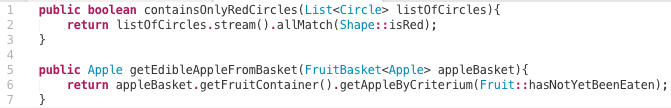
\includegraphics[width=1\columnwidth]{img/type2}
  \caption{Example of a type 2 clone.}
  \label{fig:type2}
\end{figure}

Looking at the example in listing \ref{fig:type2}, we see an example of a type 2 clone that poses no harm to the design of the system. Both methods are, except for their matching structure, completely different in functionality. They operate on different types, call different methods, return different things, etc. Having such a method flagged as a clone does not provide much useful information.

When looking at refactoring, type 2 clones can be very difficult to refactor. For instance if we have variability in types, the code can describe operations on two completely dissimilar types. Type 2 clones do not differentiate between primitives and objects, which makes the these clones often not so useful for refactoring purposes.

\subsection{Type 3 clones}
Type 3 clones are \textit{copied fragments with further modifications. Statements can be changed, added or removed in addition to variations in identifiers, literals, types, layout and comments} \cite{roy2007survey}. Detection of clones by this definition can be very hard, as it may be hard to detect whether a fragment was copied in the first place if it was severely changed. Because of this, most clone detection implementations of type 3 clones work on basis of a similarity threshold \cite{svajlenko2014evaluating, cordy2011nicad}. This similarity threshold has been implemented in different ways: textual similarity (for instance using levenshtein distance) \cite{lavoie2011automated}, token-level similarity of statement-level similarity.

Having a definition that allows for any change in code poses serious challenges on refactoring. A levenshtein distance of one can already change the meaning of a code fragment significantly, for instance if the name of a type differs by a character (and thus referring to different types).

\section{Refactoring-oriented clone types}
To resolve the shortcomings of clone types as outlined in the previous section, we propose alternative definitions for clone types to be directed at detecting clones that can and should be refactored. We have named these clones type 1R, 2R and 3R clones. These definitions share similarities with the literature definitions, the number of each type corresponds with the clone type it is modeled after. The ``R'' stands for refactoring-oriented (and may be less suitable for other analyses).

\subsection{Type 1R clones} \label{chap:type1rclones}
We propose an alternative definition of type 1 clones. This definition requires cloned fragments to be not just textually equal, but also functionally equal. Although requiring fragements to be functionally equal, type 1R clones do not allow for change in implementation (like type 4 clones). We check functional equality of two fragments by validating the equality of the fully qualityfied identifier for referenced types, methods and variables. Type 1R clones are always a subset of type 1 clones.

\subsubsection{Referenced Types}
Many object-oriented programming languages (like Java, Python, C\#) require the programmer to import a type (or the class in which it is declared) before it can be used. Based on what is imported, the meaning of the name of a type can differ. For instance, if we import \texttt{java.util.List}, we get the interface which is implemented by all list datastructures in Java. However, importing \texttt{java.awt.List}, we get a listbox GUI component for the Java Abstract Window Toolkit (AWT). Because of this, for type 1R clones, we compare the fully qualified identifier for all referenced types.

\subsubsection{Called methods}
A codebase can have several methods with the same name. The implementation of these methods might differ. When we call two methods with an identical name, we can in fact call different methods. This is another reason that textually identical code fragements can differ functionally.

Because of this, for type 1R clones, we compare the fully qualified method signature for all method references. A fully qualified method signature consists of the fully qualified name of the method, the fully qualified type of the method plus the fully qualified type of each of its arguments. For instance, an \texttt{eat} method could become \texttt{java.lang.Boolean com.simonbaars.fruitgame.Apple.eat(java.util.List<com.simonbaars.fruitgame.tools.Tool>)}.

\subsubsection{Variables}
In typed programming languages, each variable declaration should declare a name and a type. When we reference a variable, we only use its name. If, in different code fragments, we use variables with the same name but different types, the code can be functionally unequal but still textually equal. As an example, see the code in figure \ref{lst:type1variables}.

\begin{figure}[H]
  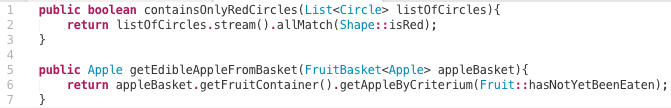
\includegraphics[width=1\columnwidth]{img/type2}
  \caption{Variables with different types but the same name.}
  \label{fig:type1variables}
\end{figure}

The body of both methods in figure \ref{lst:type2variables} is equal. However, their functionality is not. The first method adds two numbers together and the other concatenates an integer to a String.

For type 1R clones variable references should be compared by both type and name.

\begin{itemize}
  \item \textbf{Compare the equality of the fully qualified method signature for method references.} If an identifier is fully qualified, it means we specify the full location of its declaration (e.g. \texttt{com.simonbaars.fruitgame.Apple} for an \texttt{Apple} object). This way we can validate whether two method references, like method calls, are functionally equal. In the method signature, not only the fully qualified identifier of the method should be considered, but also the type of all its arguments. This way we can be sure that two potentially cloned method references do not point to overloaded variants (in a case that the data type of arguments is overloaded).
  \item \textbf{Compare the equality of the fully qualified identifier for type references.} This way we can be sure that two referenced types are actually equal, and that they are not just two types with the same name.
  \item \textbf{Compare the equality of the fully qualified identifier for variable usages.} Two cloned lines might use a variable with the same name, but different types. This might pose serious challenges on refactoring, as the variables might not concern the same object or primitive. To check this, we need to track the declaration of variables and from this infer the fully qualified identifier of its type.
\end{itemize}

\section{Type 2R clones}
Type 2 clones allow any change in identifiers, literals, types, layout, and comments. For refactoring purposes, this definition is unsuitable; if we allow any change in identifiers, literals, and types, we cannot distinguish between different variables, different types and different method calls anymore. This could render two methods that have an entirely different functionality as clones. Refactoring such clones can be harmful instead of helpful.

We tackle these problems with type 2R clones to be able to detect such clones that can and should be refactored. Type 1R clones are a subset of type 2R clones. All rules that apply to type 1R clones also apply to type 2R clones. However, type 2R clones

\begin{itemize}
  \item \textbf{Considering types:} Type 2 clones do not consider types. However, this can make a code fragment very hard to refactor, as different types can describe different functional concepts. Because of this, we propose that type 2R clones should consider types like type 1R clones do.
  \item \textbf{Having a distinction between different variables:} For type 2 clones, no identifiers would be taken into account. We agree that a difference in identifiers may still result in a harmful clone, but we should still consider the distinction between different variables. For instance, if we call a method like this: \texttt{myMethod(var1, var2)}, or call this method like this: \texttt{myMethod(var1, var1)}. Even if the variables have the same type, the distinction between the variables is important to ensure the functionality is the same after refactoring.
  \item \textbf{Defining a threshold for variability in literals:} For type 2 clones no literals would be taken into account. We agree, as when refactoring the clone (for example by extracting a method), we can turn the literal into a method parameter. However, we would argue that thresholds matter here. How many literals may differ for the segment still to be considered a clone with another segment? We need to define a threshold to be sure that, by refactoring, we are not replacing a code fragment by a worse maintainable design.
  \item \textbf{Consider method call signatures and define a threshold for variability in method calls:} As type-2 clones allow changes in identifiers, also the names of called methods may vary. However, because of this, completely different methods can be called in cloned fragments as a result. This poses serious challenges on refactoring and makes it more disputable whether such a clone is harmful for the maintainability of the code. This is because different method identifiers can describe a completely different functionality. Therefore, we suggest considering the call signatures of cloned methods when they are compared. We can allow variability in the rest of method identifiers by passing the function as a parameter. To limit the amount of parameters required we also recommend defining a threshold for variability in method call expressions, so only a limited number of method calls can vary.
\end{itemize}

\section{Type 3R clones}
Type 3 clones are even more permissive than type 2 clones, allowing added and removed statements. For these clones, thresholds matter a lot to make sure that not the whole project is detected as a clone of itself. The main question for this study regarding type 3 clones is: \textit{``how can we refactor type 3 clones while improving the design?''}.

Clone instances in type 3 clones are almost always different in functionality. As we have to ensure equal functionality after refactoring the clone, we have to wrap the difference in statements between the clone instances in conditional blocks. We can then pass a variable to indicate which path should be taken through the code (either a boolean or an enumeration). Such a refactoring would make added statements that are contiguous less harmful for the design than added statements that are scattered throughout the cloned fragment.

We also argue that statements that are not common between two clone instances, should not count towards the size of the clone (and thus towards the threshold which determines whether the clone will be taken into account). As for the detection of type 3 clones, we think the easiest opportunity to detect these clones is to consider it as a postprocessing step after clone detection. By trying to find short gaps between clones, we can find opportunities to refactor clone classes into a single type 3 clone class. The amount of statements that this ``short gap'' can maximally span should be dependent on a threshold value.

\section{The challenge of detecting these clones}\label{chap:challenge}
To detect each type of clone, we need to parse the fully qualified identifier of all types, method calls and variables. This comes with serious challenges, regarding both performance and implementation. Also, to be able to parse all fully qualified identifiers, and trace the declarations of variables, we might need to follow cross file references. The referenced types/variables/methods might even not be part of the project, but rather of an external library or the standard libraries of the programming language. All these factors need to be considered for the referenced entity to be found, on basis of which a fully qualified identifier can be created.

\section{Unifying the types}
In this chapter we have proposed refactoring-oriented definitions using the type 1, 2 and 3 clone definitions from literature as a baseline. In literature, these definitions are mainly aimed towards reasoning about duplication in source code. When considering these types for refactoring, the goal becomes slighly different. Because of this, having separate clone type definitions does not have any value. Rather, we need a single clone type definition by which we can detect all clones that can and should be considered for refactoring.

Because of this, the ultimate goal would be not to consider type 1R, 2R and 3R separately, but together. However, this is dependent on good thresholds for the type 2R variability and type 3R gap size. Because of this, we have dedicated section \ref{sec:thresholds} to performing measurements to find good thresholds. The ultimate goal is to have a single unified definition of clones that can and should be refactored. Although it will be next to impossible to define such a definition and its corresponding thresholds that does not detect false positives. However, we strive to find at least a near-optimal set of thresholds regarding the type definitions proposed in this chapter.

\section{Suitability of existing Clone Detection Tools towards our refactoring purposes}
\label{ch:tool-overview}
We conducted a short survey on (recent) clone detection tools that we could use to analyze refactoring possibilities. The results of our survey are displayed in table~\ref{table:dettools}. We chose a set of tools that are open source and can analyze a popular object-oriented programming language. Next, we formulate the following four criteria by which we analyze these tools:
\begin{enumerate}
    \item \textbf{Should find clones in any context.} Some tools only find clones in specific contexts, such as only method-level clones. We want to perform an analysis on all clones in projects to get a complete overview.
\item \textbf{Should find all clones in created control projects.} We assembled a number of test projects to assess the validity of clone detection tools. On basis of this, we checked whether clone detection tools can correctly find clones in diverse contexts.
\item \textbf{Can analyse resolved symbols.} When detecting clones for refactoring purposes, it is important that clone instances can be refactored. Sometimes, textual equality between code fragments does not imply that these can be refactored (this is described more elaborately in section \ref{chap:type1clones}). Because of this, we want to use a clone detection tool that can analyze such structures.
\item \textbf{Extensive detection configuration.} We aim to exclude expressions/statements from matching (more about our rationale in section~\ref{chap:clonetypes}). To achieve this, the tool needs to be able to allow those threshold changes. This can be either through simple changes of the source code, or by using some configuration file.
\end{enumerate}

\begin{table}[H]
 \begin{center}
  \caption{Our survey on clone detection tools.} \label{table:dettools}
  \medskip
\begin{tabular}{|l|l|l|l|l|l|}
\hline
\textbf{Clone Detection Tool} & \textbf{(1)} & \textbf{(2)} & \textbf{(3)} & \textbf{(4)} \\ \hline
Siamese \cite{ragkhitwetsagul2019siamese} &  &             &             & \checkmark            \\ \hline
NiCAD \cite{roy2008nicad, cordy2011nicad} & \checkmark                             & \checkmark            &             &             \\ \hline
CPD \cite{roy2009comparison} & \checkmark & \checkmark            &             &             \\ \hline
\begin{tabular}[c]{@{}l@{}}CCFinder \cite{kamiya2002ccfinder}\\ D-CCFinder \cite{livieri2007very}\end{tabular} & \checkmark  & \checkmark   &    &   \\ \hline
CCFinderSW \cite{semura2017ccfindersw}   & \checkmark     &             &             & \checkmark            \\ \hline
\begin{tabular}[c]{@{}l@{}}SourcererCC \cite{sajnani2016sourcerercc}\\ Oreo \cite{saini2018oreo}\end{tabular} & \checkmark    &             &             & \checkmark            \\ \hline
BigCloneEval \cite{svajlenko2016bigcloneeval}  & \checkmark  & \checkmark   &             &             \\ \hline
Deckard \cite{jiang2007deckard} & \checkmark   &             & \checkmark            &             \\ \hline
Scorpio \cite{higo2013revisiting, kamalpriya2017enhancing} & \checkmark   &     & \checkmark  & \checkmark   \\ \hline
\end{tabular}
\end{center}
\end{table}

None of the state-of-the-art tools we identified implement all our criteria, so we decided to implement our own clone detection tool: CloneRefactor\footnote{CloneRefactor (WIP) is available on GitHub: \url{https://github.com/SimonBaars/CloneRefactor}. This repository contains all scripts that were used to retrieve the data that is displayed in this paper.}.

\chapter{Evaluation setup}
In this chapter we describe the setup we use for our experiments. Our most prominent contribution is the proposal of a tool called CloneRefactor. This tool allows us to map clones with all clone definitions as described in chapter \ref{chap:clonetypes}.

All data for our experiments, as displayed in chapter \ref{ch:results}, is measured over a corpus of Java projects. In this chapter we will explain how we prepared this corpus.

\section{CloneRefactor}
CloneRefactor is the name of our clone detection and refactoring tool. It features the following novel functions:
\begin{itemize}
  \item Detection of clone classes rather than clone pairs.
  \item A novel detection method, aimed at extensibility.
  \item Detection of refactoring-oriented clone types, in addition to the literature clone types.
  \item Allows for automated refactoring of a subset of the detected duplication issues.
\end{itemize}
In this section we describe our approach and rationale for the design decisions regarding this tool.

\subsection{JavaParser}
A very important design decision for CloneRefactor is the usage of a library named JavaParser \cite{tomassetti2017javaparser}. JavaParser is a Java library which allows to parse Java source files to an abstract syntax tree (AST). JavaParser allows to modify this AST and write the result back to Java source code. This allows us to apply refactorings to the detected problems in the source code.

Integrated in JavaParser is a library named SymbolSolver. This library allows for the resolution of symbols using JavaParser. For instance, we can use it to trace references (methods, variables, types, etc) to their declarations (these referenced identifiers are also called ``symbols''). This is very useful for the detection of our refactoring-oriented clone types, as they make use of the fully qualified identifiers of symbols.

In order to be able to trace referenced identifiers SymbolSolver requires access to not only the analyzed Java projects, but also all its dependencies. This requires us to include all dependencies with the project. Along with this, SymbolSolver solves symbols in the JRE System Library (the standard libraries coming with every installation of Java) using the active Java Virtual Machine (JVM). This has a big impact on performance efficiency.

Because of the requirement of symbol resolution, the refactoring-oriented clone types are less suitable for large scale clone analysis.

\subsection{Clone Detection}
To detect clones, CloneRefactor parses the AST aqcuired from JavaParser to an unweighted graph structure. On basis of this graph structure, clones are detection. Dependent on the type of clones being detected, transformations may be applied. The way in which CloneRefactor was designed does not allow for several clone types to be detected simultaneously, in accordance with our clone type philosophy as described in chapter \ref{section:clonephilosophy}.

\subsection{Type specific transformations}

\section{The corpus}\label{chap:corpus}
For our measurements we use a large corpus of open source projects \cite{githubCorpus2013}. This corpus has been assembled to contain relatively higher quality projects. Also, any duplicate projects were removed from this corpus. This results in a variety of Java projects that reflect the quality of average open source Java systems and are useful to perform measurements on.

As indicated in chapter \ref{chap:challenge} CloneRefactor requires all libraries of software projects we test. As these are not included in the used corpus \cite{githubCorpus2013}, we decided to filter the corpus to only include Maven projects. Maven is a build automation tool used primarily for Java, and works on basis of an \texttt{pom.xml} file to describe the projects' dependencies. As no \texttt{pom.xml} files are included in the corpus, we cloned the latest version of each project in the corpus. We then removed each project that has no \texttt{pom.xml} file. As a final step, we collected all dependencies for each project by using the \texttt{mvn dependency:copy-dependencies -DoutputDirectory=lib} Maven command, and removed each project for which not all dependencies were available (due to non-Maven dependencies being used or unsatisfiable dependencies being referenced in the \texttt{pom.xml} file).

Some general data regarding this corpus is displayed in Table \ref{table:general}.

\begin{table}[H]
  \begin{center}
  \caption{General results for GitHub Java projects corpus \cite{githubCorpus2013}.} \label{table:general}
  \medskip
\begin{tabular}{|l|l|}
\hline
Amount of projects                                                                                      & 1,361      \\ \hline
\begin{tabular}[c]{@{}l@{}}Amount of lines (excluding\\whitespace, comments and newlines.)\end{tabular} & 1,414,996  \\ \hline
Amount of statements/declarations                                                                       & 1,212,189  \\ \hline
\begin{tabular}[c]{@{}l@{}}Amount of tokens (excluding\\whitespace, comments and newlines.)\end{tabular} & 11,643,194 \\ \hline
\end{tabular}
\end{center}
\end{table}
